\documentclass[11pt,a4paper]{report}
 \usepackage[francais]{babel}
 \usepackage[utf8]{inputenc}
\usepackage[T1]{fontenc}
\usepackage{graphicx}
\usepackage{subfig}
\usepackage{caption}
\usepackage{amssymb}
\usepackage{amsmath}
\usepackage{listings}
\usepackage{scrextend}
\usepackage{xcolor}
\usepackage{hyperref}
\usepackage[toc,page]{appendix}
\usepackage[margin=2 cm]{geometry}
%\usepackage[symbols]{circuitikz}
%\usepackage{tikz}
\lstset{language=R,
basicstyle=\fontfamily{pcr}\selectfont\footnotesize\color{black},
frame = single}
\graphicspath{ {./figures/} }


\date{2018}

\begin{document}

\tableofcontents

\chapter*{Définition de la dérive conceptuelle}

On peut définir plusieurs type de dérives avec la formule de bayes.
$$
P(y \mid X)=\frac{ P(y)P(X\mid y)}{P(X)}
$$
 
 On voit avec la figure 1, différents types de dérives. La dérive (a) vient d'un changement de $P(y)$, (b) est causé par un changement de $P(X\mid y)$ et (c) par $P(y \mid X)$. Les dérives illustrées par (b) et (c) sont celles qui portent atteinte le plus au modèle. On peut aussi avoir d'autres dérives détaillé dans les exemples.

\begin{figure}[h]
\caption{Différents types de dérive}
\centering
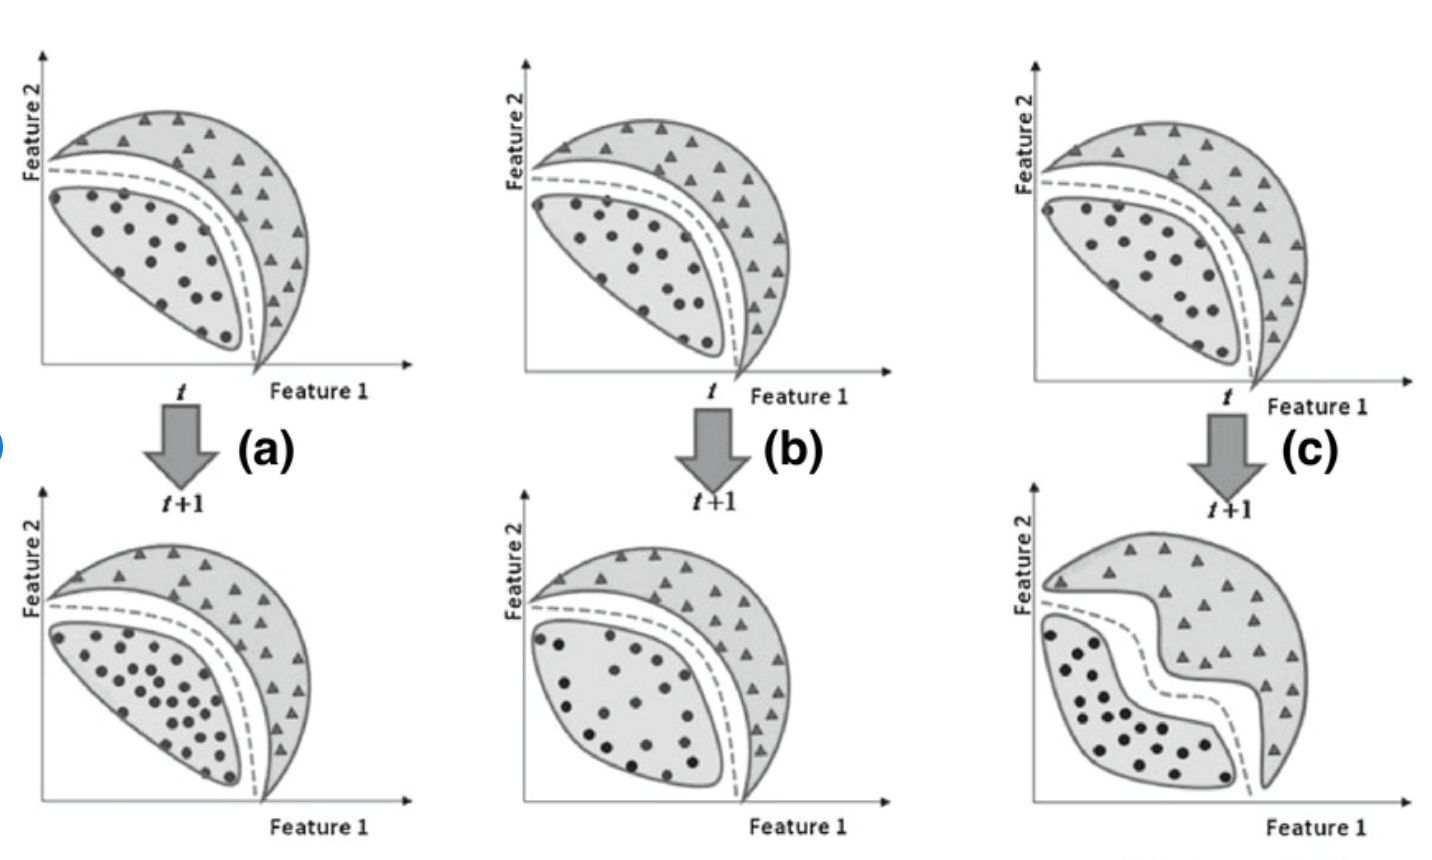
\includegraphics[width=0.6\textwidth]{different_types_of_drift}
\end{figure}

La dérive de type (a) peut être modeste dans la baisse de performance. Mais quand le modèle ne peut pas trouver une frontière sans faire du sur apprentissage, où dans certaines zone où la frontière laisse une zone d'incertitude, alors cette type de dérive peut être problématique.

Exemples:
\begin{list}{•}
\item[Changement de $P(y)$] Si on cherche à prédire les transactions frauduleuses, et petit à petit, leurs proportions augmentent, il y a de plus en plus de fraudes sans que leurs définitions changent.
\item[Changement de $P(X\mid y)$] Toujours dans le cas de la détections des fraudes, un nouveau type de fraude est mis en œuvre, de nouveaux types de transaction apparaissent, ce sont des fraudes.
\item[Changement de $P(y \mid X)$] Un nouveaux dispositif de sécurité est mis en place, seulement certains sites web sont autorisés pour les transactions, des transactions qui était normales sont maintenant des fraudes.
\item[Changement du vecteur $X$] 
\end{list}


\begin{figure}
\centering
\begin{minipage}{.5\textwidth}
  \centering
  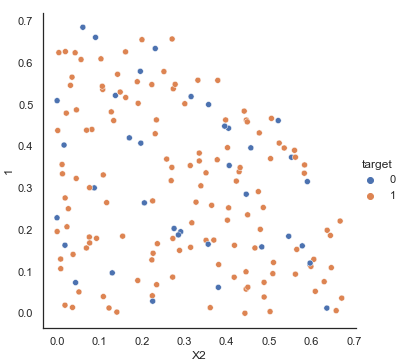
\includegraphics[width=0.7\linewidth]{P_x_before.png}
  \captionof{figure}{Concept à l'instant $t$}
  \label{fig:test1}
\end{minipage}%
\begin{minipage}{.5\textwidth}
  \centering
  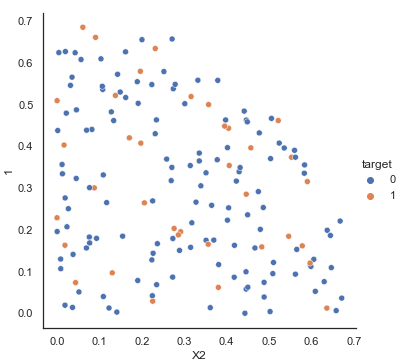
\includegraphics[width=0.7\linewidth]{P_x_later.png}
  \captionof{figure}{Concept à l'instant $t+\Delta t$}
  \label{fig:test2}
\end{minipage}
\end{figure}


\newpage

Les articles de recherche peuvent être séparés en deux catégories. Ceux qui ce focalisent sur la création d'un algorithme, ou d'un shéma d'apprentissage robuste a la dérive. Et ceux qui développent des méthodes faites pour détecter la dérive, sans se préocupper du modèle.


\section*{Évaluation des méthodes}

Il existe plusieurs forme d'évaluation des méthodologies. 
\begin{itemize}
\item Dans le cas de développement d'un nouvel algorithme, on peut comparer la qualité de ses prédiction sur un certains nombre de jeux de données (de synthèse où réel) détaillés dans un autre document.
\item Dans le cas d'une méthode de détection de dérive, on peut regarder le nombre d'observations nécessaires avant la détection de celle-ci.
\end{itemize}

\chapter{On peut répartir les différentes méthodologies en plusieurs catégories.}
\section{Méthodes utilisant un test statistique}

\subsection{Learning from Time-Changing Data with Adaptive Windowing}
\subsubsection{A Bifet, R Gavalda , 2007}

\paragraph{Type de Dérive :} $P(X\mid y)$ et $P(y \mid X)$
\paragraph{Quelles informations utilisées dans la détection :} Données
\paragraph{Quel type de détection :} Détection de dérive. Adaptable à tout modèles.

\paragraph{Mots clefs} Tests Statistiques, Détection sur score de modèle.

\paragraph{Mots clefs :} ADWIN

\paragraph{Résumé :} Un algorithme de sélection de fenêtre d’apprentissage est présenté. L’algorithme conserve les n plus récentes observations dans une fenêtre $W$ de taille $n$ avant de la séparer en deux parties $W_1$ et $W_2$ de taille $n_1$ et $n_2$ tel que $n_1+n_2=n$. 

Avec $m=\frac{1}{1 / n_{0}+1 / n_{1}} \text { (moyenne harmonique de } n_{0} \text { et } n_{1} )  $; $\delta^{\prime}=\frac{\delta}{n} \text{ et } $ $ \quad \epsilon_{c u t}=\sqrt{\frac{1}{2 m} \cdot \ln \frac{4}{\delta^{\prime}}}$. 

Tant que l'on observe pas $\left|\hat{\mu}_{W_{0}}-\hat{\mu}_{W_{1}}\right| \geq \epsilon_{c u t}$ où $\hat{\mu}_{W_{0}}$ est la moyenne de la fenêtre $W_0$ et $\hat{\mu}_{W_{1}}$ celle de $W_1$, on supprime les observations les plus anciennes

\paragraph{À quelle(s) problématique(s) l'article répond ?} Détection d'une dérive, sélection des observations correspondant au concept le plus récent.

\paragraph{Quelles sont les pistes à explorer et ont-elles  été explorées par d'autres articles ?} Utiliser ADWIN pour séparer les données en concepts différents $C_1, C_2, ... C_i$ avec des statistiques telles que la moyenne, la variance, les quantiles... Cela permettrait, quand un nouveau concept apparaîtrait de vérifier si l'on ne dispose pas d'autres instances de ce concept dans le cas d'un concept récurrent.

Implémentation : \url{https://scikit-multiflow.readthedocs.io/en/stable/api/generated/skmultiflow.drift_detection.ADWIN.html#skmultiflow.drift_detection.ADWIN}










\subsection{Concept drift detection based on Fisher’s Exact test}
\subsubsection{Danilo Rafael de Lima Cabral, Roberto Souto Maior de Barros, 2018}

\paragraph{Type de Dérive :} $P(X\mid y)$ et $P(y \mid X)$
\paragraph{Quelles informations utilisées dans la détection :} Prédictions, classes réelles
\paragraph{Quel type de détection :} Détection de dérive. Adaptable à tout modèles.

\paragraph{Mots clefs :} Tests Statistiques, Détection sur score de modèle.

\paragraph{Résumé :}
L'article propose trois méthodes de détection de dérive à partir du test de Fischer fait sur les prédictions du modèle, les variantes sont en partie faites pour réduire le coût calculatoire. Les différences entres les méthodes sont les tests statistiques et la manière dont ils sont utilisés. Dans les trois cas, on suppose que l'on dispose des prédictions du modèle et de la vérité. On sépare les prédictions en 2 ensembles, les plus récentes et les anciennes, on va ensuite, à l'aide de tests statistiques regarder si une différence de distribution apparait conséquence d'une dérive. 

FPDD utilise le test de Fischer quand le nombre d'erreurs où de prédicitions justes est faible (inférieur à 5) et utilise le test de l'hypothèse des proportion égale utilisé par la méthode STEPD le cas échéant. $T\left(r_{0}, r_{r}, n_{o}, n_{r}\right)=\frac{\left|r_{0} / n_{o}-r_{r} / n_{r}\right|-0.5 \times\left(1 / n_{o}+1 / n_{r}\right)}{\sqrt{\hat{p} \times(1-\hat{p}) \times\left(1 / n_{o}+1 / n_{r}\right)}}$.

FSDD utilise le test de Fischer quand le nombre d'erreurs où de prédicitions justes est inférieure à 5 et utilise le test du chi deux le cas échéant.

FTDD utilise le test de Fischer exclusivement.

Les trois méthodes sont testées avec plusieurs jeux de données contre DDM, ECDD, SEED, FHDDM, STEPD et sortent avec en moyenne de meilleurs résultats.
\paragraph{À quelle(s) problématique(s) l'article répond ?} Amélioration du temps de calcul et des performances de plusieurs méthodes

\paragraph{Quelles sont les pistes à explorer et ont-elles été explorées par d'autres articles ?} Il reste à explorer plus de tests statistiques et étudier une possible combinaison, càd l'utilisation de plusieurs tests en simultané et un méta modèle. Expérimenter l'impact de la taille des fenêtres d'observations prises en compte (elles sont brièvement étudiées).









\subsection{Detecting Concept Drift Using Statistical Testing}
\subsubsection{Kyosuke Nishida and Koichiro Yamauch, 2007}

\paragraph{Type de Dérive :} $P(X\mid y)$ et $P(y \mid X)$
\paragraph{Quelles informations utilisées dans la détection :} Prédictions, classes réelles.
\paragraph{Quel type de détection :} Détection de dérive. Adaptable à tout modèles.

\paragraph{Mots clefs} Tests Statistiques, Détection sur score de modèle.

\paragraph{Résumé :} L'article propose une méthode de détection de dérive à partir d'un test. On suppose que l'on dispose des prédictions du modèle et de la vérité. On sépare les prédictions en 2 ensembles, les plus récentes et les anciennes, on va ensuite, à l'aide de la statistique $$T\left(r_{0}, r_{r}, n_{o}, n_{r}\right)=\frac{\left|r_{0} / n_{o}-r_{r} / n_{r}\right|-0.5 \times\left(1 / n_{o}+1 / n_{r}\right)}{\sqrt{\hat{p} \times(1-\hat{p}) \times\left(1 / n_{o}+1 / n_{r}\right)}}$$ rejeter où accepter l'hypothèse de même distribution. 

\paragraph{À quelle(s) problématique(s) l'article répond ?} L'article propose une méthodologie de détection de dérive sur les scores des modèles.

\paragraph{Quelles sont les pistes à explorer et ont-elles été explorées par d'autres articles ?} La technique laisse à désirer en présence de dérive graduelle. Taille de la fenêtre.










\subsection{Learning with Drift Detection}
\subsubsection{João Gama, Pedro Medas, Gladys Castillo, Pedro Rodrigues, 2004}

\paragraph{Type de Dérive :} $P(X\mid y)$ et $P(y \mid X)$
\paragraph{Quelles informations utilisées dans la détection :} Prédictions, classes réelles.
\paragraph{Quel type de détection :} Détection de dérive. Adaptable à tout modèles.

\paragraph{Mots clefs}

\paragraph{Résumé :} Les auteurs introduisent le terme de contexte. Selon eux, au sein d'un contexte la distribution des données est stationnaire. Lors de la présence d'une dérive, celle-ci est traduite par un changement de contexte, où la distribution est stationnaires, mais plus où moins différentes que la précédente. Le but de la méthode développée ici est d'utiliser des intervalles de confiance de la loi normale appliqué aux erreurs faites par le modèle pour détecter une dérive. L'erreur devant logiquement diminuer au fur et à mesure que le modèle dispose de données d'entraînement faisant l'hypothèse que la distribution sous-jacente est la même, quand celle-ci augmente au delà d'un certain seuil, on est en présence d'une dérive.

\paragraph{À quelle(s) problématique(s) l'article répond ?} L'article propose une méthodologie de détection de dérive sur les scores des modèles.

\paragraph{Quelles sont les pistes à explorer et ont-elles  été explorées par d'autres articles ?} L'article ne compare pas les autres travaux, mais compare les différences de performances avec et sans la méthodologie.







\subsection{Concept drift detection and adaptation with Hierarchical Hypothesis Testing}
\subsubsection{Shujian Yu, Zubin Abraham, Heng Wang; 2019}

\paragraph{Type de Dérive :} $P(X\mid y)$ et $P(y \mid X)$
\paragraph{Quelles informations utilisées dans la détection :} Prédictions, classes réelles.
\paragraph{Quel type de détection :} Détection de dérive. Adaptable à tout modèles.

\paragraph{Mots clefs} Statistical Tests, Hierarchical, Adaptive Training

\paragraph{Résumé :} Afin de détecter une dérive conceptuelle de manière stable, les auteurs mettent en place une méthodologie à deux niveaux. Un premier niveau détecte à travers l'instabilitée de 4 métriques relatant les performances du modèle, une dérive. Les auteurs en utilise 4 car l'utilisation d'une seule, comme dans d'autres méthodologies exisantes, ne permet pas l'obtention d'un délais de détection rapide et de précision forte.

Si une détection est relevée, alors un deuxième test est fait en comparant les performances du modèle entraîné sur les données d'avant la dérive et d'après. Les auteurs utilisent également une version adaptable de l'algorithme SVM permettant l'utilisation des données du concept précédent afin d'améliorer les performances du nouveau modèle, peu d'exemples d'entraînements étant disponibles après détéction d'un nouveau concept.

\paragraph{À quelle(s) problématique(s) l'article répond ?} Les techniques développées permettent une détection plus rapide de la dérive. Le modèle adaptable permet de bonnes performances malgrès le nombre faible d'observations.

\paragraph{Quelles sont les pistes à explorer et ont-elles  été explorées par d'autres articles ?} Rendre d'autres algorithmes Adaptables (Lire  reférence 54).








\subsection{Online and Non-Parametric Drift Detection Methods Based on Hoeffding’s Bounds}
\subsubsection{Frias-Blanco, Campo-Avila; 2015}

\paragraph{Type de Dérive :} $P(X\mid y)$ et $P(X)$
\paragraph{Quelles informations utilisées dans la détection :} Prédictions, classes réelles.
\paragraph{Quel type de détection :} Détection de dérive. Adaptable à tout modèles.

\paragraph{Mots clefs} Statistical Tests, Hierarchical, Adaptive Training

\paragraph{Résumé :} Pour détecter un dérive au sein des données d'entraînement, les auteurs mettent en place deux méthodologie basé sur l'inéglité de Hoeffding.

Un première méthode utilise la moyenne comme critère de détéction, la deuxième une moyenne pondérées.

\paragraph{À quelle(s) problématique(s) l'article répond ?} Les techniques développées permettent une détection rapide de la dérive. 

\paragraph{Quelles sont les pistes à explorer et ont-elles  été explorées par d'autres articles ?}








\subsection{Wilcoxon Rank Sum Test Drift Detector}
\subsubsection{Roberto Souto Maior de Barro; 2017}

\paragraph{Type de Dérive :} $P(y\mid X)$
\paragraph{Quelles informations utilisées dans la détection :} Prédictions
\paragraph{Quel type de détection :} Détection de dérive. Adaptable à tout modèles.

\paragraph{Mots clefs} Statistical Tests

\paragraph{Résumé :} Pour détecter un dérive au sein des données les auteurs vont effectuer un test de Wilcoxon sur les prédictions du modèle deux fenêtres, une ancienne et une récente.
Contrairement à STEPD, la taille de l'ancienne fenêtre est limité.

\paragraph{À quelle(s) problématique(s) l'article répond ?} Les techniques développées permettent une détection rapide de la dérive. 

\paragraph{Quelles sont les pistes à explorer et ont-elles  été explorées par d'autres articles ?}








\subsection{Efficient Handling of Concept Drift and ConceptEvolution over Stream Data}
\subsubsection{Roberto Souto Maior de Barro; 2017}

\paragraph{Type de Dérive :} $P(y\mid X)$,  Nouvelles classes
\paragraph{Quelles informations utilisées dans la détection :} 
\paragraph{Quel type de détection :} Détection de dérive. Adaptable à tout modèles à base de cluster.

\paragraph{Mots clefs} Statistical Tests

\paragraph{Résumé :} 
L'algorithme maintient à jour un ensemble de modèle de classification de type k plus proches voisins. 
À l'arrivé d'un nouvel exemple, celui-ci est prédit, mais, si il se trouve trop loin des clusters existant, alors, il est considéré comme un outlier et est stocké dans un buffer. Quand il y a assez d'exemples dans le buffer, on calcule une métrique pour chaque couple (exemple, modèle de l'ensemble). Si des exemple ne peuvent pas être rattaché à des clusters, alors on a emergence d'une nouvelle classe et ceux ci sont incorporé à un nouveau modèle. 

Dès qu'une nouvelle instance doit est prédite, un score de confiance en la prediction est également calculé et stocké. S'il y a une détection de changement de distribution dans la série de valeurs de confiance des prédiction alors on à une dérive. La taille de la fenêtre est ajusté, certains exemples sont selectionné basé sur leur score de confiance et leurs labels sont récupérés (Comment ? Pas pratique) et un modèle est entrainé avec ceux-ci et remplace le plus vieux modèle de l'ensemble..

\paragraph{À quelle(s) problématique(s) l'article répond ?} L'emergence de nouvelle classe.

\paragraph{Quelles sont les pistes à explorer et ont-elles  été explorées par d'autres articles ?}





\subsection{RCD: A Recurring Concept Drift Framework}
\subsubsection{Gonc, Campo-Avila; 2013}

\paragraph{Type de Dérive :} $P(X\mid y)$ et $P(X)$
\paragraph{Quelles informations utilisées dans la détection :} Prédictions, classes réelles.
\paragraph{Quel type de détection :} Détection de dérive. Adaptable à tout modèles.

\paragraph{Mots clefs} Statistical Tests, Hierarchical, Adaptive Training

\paragraph{Résumé :} Pour détecter un dérive au sein des données d'entraînement, les auteurs mettent en place deux méthodologie basé sur l'inéglité de Hoeffding.

Un première méthode utilise la moyenne comme critère de détéction, la deuxième une moyenne pondérées.

\paragraph{À quelle(s) problématique(s) l'article répond ?} Les techniques développées permettent une détection rapide de la dérive. 

\paragraph{Quelles sont les pistes à explorer et ont-elles  été explorées par d'autres articles ?}







\subsection{Active learning approach to concept drift problem}
\subsubsection{BARTOSZ; 2010}

\paragraph{Type de Dérive :} $P(X\mid y)$ et $P(X)$
\paragraph{Quelles informations utilisées dans la détection :} ancien labels, vecteur X
\paragraph{Quel type de détection :} Quand récupérer des labels. Adaptable à tout modèles.

\paragraph{Mots clefs :} Semi-supervisé

\paragraph{Résumé :} Ici les auteurs proposent un algorithme permettant de décider quand il est nécessaire de demander les classes réelles des instances pour un réentrainement basé sur des mesures de distance.

\paragraph{À quelle(s) problématique(s) l'article répond ?} Drift dans un contexte semi-supervisé.

\paragraph{Quelles sont les pistes à explorer et ont-elles  été explorées par d'autres articles ?}








\subsection{Concept Drift Detection: Dealing with Missing Values via Fuzzy Distance Estimations}
\subsubsection{Liu, Lu; 2020}

\paragraph{Type de Dérive :} $P(X\mid y)$ et $P(X)$
\paragraph{Quelles informations utilisées dans la détection :} vecteur X
\paragraph{Quel type de détection :} Surtout pour avoir une imputation de valeur manquante non gênante dans la détection de dérive.

\paragraph{Mots clefs :} 

\paragraph{Résumé :} Ici les auteurs proposent un algorithme un algorithme permettant l'imputation de valeurs manquantes. Cette imputation se fait de façon à garder la variance des données. En effet, on imagine que remplacer les valeurs manquantes par la moyenne en présence de dérive, ne marche pas bien avec ADWIN par exemple.

\paragraph{À quelle(s) problématique(s) l'article répond ?} Valeurs manquantes

\paragraph{Quelles sont les pistes à explorer et ont-elles  été explorées par d'autres articles ?}









\subsection{Handling adversarial concept drift in streaming data}
\subsubsection{Tegjyot Singh Sethi , Mehmed Kantardzic, 2017}

\paragraph{Mots clefs}  adversarial concept drift 

\paragraph{Résumé :} A lire.

\paragraph{À quelle(s) problématique(s) l'article répond ?}

\paragraph{Quelles sont les pistes à explorer et ont-elles  été explorées par d'autres articles ?}

















\newpage












\section{Méthodes à base de modèles}
\subsection{Tracking recurring contexts using ensemble classifiers: an application to email filtering}
\subsubsection{Ioannis Katakis, Grigorios Tsoumakas, Ioannis Vlahavas, 2009}

\paragraph{Type de Dérive :} $P(X\mid y)$ et $P(y \mid X)$
\paragraph{Quelles informations utilisées dans la détection :} Exemples non labélisés
\paragraph{Quel type de détection :} Catégorisation de concept. Adaptable à tout modèles.

\paragraph{Mots clefs} Dérive récurrente

\paragraph{Résumé :} On suppose que les données arrivent par séries où packets, on va les projeter les données dans un espace, puis, un algorithme non supervisé va les grouper par concepts, l'espace de projection permettant de comparer les instances avec la distance euclidienne. Chaque concept différent dispose de son modèle prédictif. Quand une nouvelle série d'observations arrive, elle est projeté dans l'espace, si elle ne correspond à aucun concept, on en créé un nouveau, sinon, on score.

La projection des variables se fait comme ceci: $z_{i}=\left\{\begin{array}{l}
\left\{P_{i, j}^{v}: j=1, \ldots, m, v \in V_{i}\right\}, \quad \text { si } f_{i} \text { est nominale } \\
\left\{\mu_{i, j}, \sigma_{i, j}: j=1, \ldots, m\right\}, \quad \text { si } f_{i} \text { est numérique }
\end{array}\right.$
Et où:
$P_{i, j}^{v}=P\left(f_{i}=v \mid c_{j}\right), i \in[1, n], j \in[1, m], v \in V_{i}$. Où $V_{i}$ est l'ensemble des valeurs possible que peut prendre la variable $f_{i}$.
\paragraph{À quelle(s) problématique(s) l'article répond ?} À la projection des espaces des données dans un espace euclidien.

\paragraph{Quelles sont les pistes à explorer et ont-elles  été explorées par d'autres articles ?} L'article fait l'hypothèse que des données d'un même batch appartiennent aux mêmes concepts.







\subsection{Learning classification rules for telecom  customer call data under concept drift}
\subsubsection{Black, M., Hickey, R, 2003}

\paragraph{Type de Dérive :} $P(X\mid y)$ et $P(y \mid X)$
\paragraph{Quelles informations utilisées dans la détection :} Classes réelles.
\paragraph{Quel type de détection :} Détection de dérive, nouvel algorithme à partir d'arbre de décision.

\paragraph{Mots clefs :} Arbre de décision, 

\paragraph{Résumé :} L'article développe plusieurs versions d'une méthodologie basée sur les arbres de décisions.  On suppose que les données arrivent par batchs. Un attribut de temporalité est introduit dans le jeu de données. Un arbre de décision est fait sur le dataset. Si l’attribut de temps est présent dans les décisions, alors on a un drift. Cela permet également de voir quelles variables ont été impactées par le drift. Seul les règle émanant des branches qui se trouvent dans la branche de l’arbre de décision où un attribut temporel est présent sont supprimées. Les règles qui n’ont pas été impactées restent.

\paragraph{À quelle(s) problématique(s) l'article répond ?} Utiliser la temporalité afin de trouver les attributs en dépendant.

\paragraph{Quelles sont les pistes à explorer et ont-elles  été explorées par d'autres articles ?} Utiliser cette méthode afin de vérifier si 








\subsection{An Ensemble Approach for Incremental Learning in Nonstationary Environments}
\subsubsection{Michael D. Muhlbaier and Robi Polikar, 2007}

\paragraph{Type de Dérive :} $P(X\mid y)$ et $P(y \mid X)$
\paragraph{Quelles informations utilisées dans la détection :} Données passées
\paragraph{Quel type de détection :} Détection de dérive, nouvel algorithme d'apprentissage en ligne.

\paragraph{Mots clefs :} Online learning

\paragraph{Résumé :} L'article propose Learn$^{++}$.NSE NSE comme Non Stationnary Environment. On suppose que les données arrivent en par paquets, ou en batch. On suppose ici que les dernières données labélisées correspondent au concept le plus récent. Ainsi, à chaque fois qu'un batch de données labélisées arrive, on entraîne un nouveau modèle. On va ensuite regarder les taux d'erreurs respectifs de chaque ancien modèle sur l'ensemble des paquets de données. 

On va ensuite attribuer une pondération à chaque modèle qui va dépendre des performances de ceux-ci sur les paquets de données. L'erreur des modèles sur les paquets récents va prendre plus de d'importance que les erreurs anciennes. Dans le cas d'une dérive récurrente, on va observer le poid d'un modèle osciller.

Le résultat de cette pondération va déterminer le poid de chacun des modèles dans la prédiction à venir.


\paragraph{À quelle(s) problématique(s) l'article répond ?} L'article répond aux problèmes des dérives récurrentes.

\paragraph{Quelles sont les pistes à explorer et ont-elles été explorées par d'autres articles ?} L'article ne prend pas en compte la séparation des paquets en concepts. En effet, deux concepts peuvent arriver au sein d'un même paquet s'ils sont trop longs. S'il sont trop courts, alors les performances du modèle seront insatisfaisantes. La méthodologie utilise seulement les performances dans son discernement des concepts, un ajout de méthodes statistiques augmenterait sûrement la pertinence de la pondération. La méthodologie entraîne un modèle unique sans ce soucier des hyperparamètres.







\subsection{Data Stream Classification Guided by Clustering on Non Stationary Environments and Extreme Verification Latency}
\subsubsection{VMA Souza, DF Silva, J Gama, GE Batista , 2015}
\subsubsection{Cité 62 fois, SIAM}

\paragraph{Type de Dérive :} $P(X\mid y)$ et $P(y \mid X)$
\paragraph{Quelles informations utilisées dans la détection :} Données d'initialisation.
\paragraph{Quel type de détection :} Détection de dérive, nouvel algorithme d'apprentissage en ligne.
\paragraph{Mots clefs :} Semi-supervisé

\paragraph{Résumé :} On dispose des labels seulement lors de l'initialisation et c'est un contexte où une dérive est présente.
L'article présente une méthodologie semi-supervisée afin de prédire dans un contexte où il y a une dérive. Le contexte est un contexte de dérive incrémentale, le nombre de classes est supposé connu et ne change pas, on dispose initialement d'un nombre d'exemples labélisés.

 À l'initialisation, on va attribuer chaque exemple à un cluster selon sa classe. On aura donc autant de clusters que de classes. Les centroïdes sont calculés.
 
 On va ensuite récupérer des exemples non labélisés, utiliser k-means pour les répartir en clusters. Pour cela, lors de l'initialisation, on utilise les centroïdes des clusters précédement définis, par les classes, comme centroïdes d'initialisation. Une fois les nouveaux points répartis en clusters, on va attribuer aux instances non labélisées composant les clusters, le label du cluster de l'itération précédente qui est le plus proche. Les nouveaux exemples labelisés, on peut réentraîner le modèle sur les exemples les plus récents. 
On peut ainsi recommencer l'itération dès l'arrivé de nouveau exemples. On oscille ainsi entre classification supervisée et clustering.

\paragraph{À quelle(s) problématique(s) l'article répond ?} L'article apporte une méthode pour traiter la dérive dans un contexte semi-supervisé. Dans un contexte où les labels des observations ne sont disponibles que lors de l'initialisation.

\paragraph{Quelles sont les pistes à explorer et ont-elles  été explorées par d'autres articles ?} On peut imaginer que dans le cas d'une dérive de forte amplitude brusque, ou lors de dérives qui s'enchaînent sur une temporalité longue, le système perde en efficacité.








\subsection{A Novel Concept Drift Detection Method for Incremental Learning in Nonstationary Environmnents}
\subsubsection{Z Yang, S Al-Dahidi, P Baraldi, E Zio, 2019}

\subsubsection{Cité 4 fois, ieeexplore.ieee.org}

\paragraph{Type de Dérive :} $P(X\mid y)$ et $P(y \mid X)$
\paragraph{Quelles informations utilisées dans la détection :} Données labélisées.
\paragraph{Quel type de détection :} Détection de dérive, méthodologie adaptable à plusieurs algorithmes.
\paragraph{Mots clefs :} Semi-supervisé

\paragraph{Mots clefs :} Détection par analyse du modèle

\paragraph{Résumé :} L'article détaille une méthode qui, pour détecter la dérive, va réentrainer un modèle (ELM) Extreme Learning Machines, qui est un modèle type réseau de neurones à une unique couche cachée. Ce type de modèle à la particularité qu'il peut être actualisé avec l'arrivée de nouvelles données quel que soit leur nombre.

Une fois le modèle entraîné, à l'arrivé de nouveaux exemples labélisés, un réentrainement s'opère. La différence de poid des neurones de la couche caché du modèle réentrainé avec les poids du modèle avant réentrainement est calculée. Les auteurs développent une distance faite pour mesurer l'écart entre les poids des deux modèles.

Si cette différence est supérieure à un seuil, dont la méthodologie de détermination est détaillé dans l'article. Un calcul, tiré de travaux récents pour quantifier le nombre d'exemples labélisés nécessaires à un réentraînement efficaces du point de vue des performances prédictives et en terme de coût caclulatoire.

\paragraph{À quelle(s) problématique(s) l'article répond ?} Comment détecter une dérive avec le modèle sans regarder les performances de celui-ci ? Comment trouver le compromi idéal pour un savoir quand faire les réentraînements ?

\paragraph{Quelles sont les pistes à explorer et ont-elles  été explorées par d'autres articles ?} Utiliser une méthodologie similaire sur d'autre algorithmes prédictif, calculer une distance entre les arbres de décisions, où trouver un seuil a partir duquel un changement des coefficients de la regression linéaire indiquerait une dérive.






\subsection{Concept Drift detection and adaptation in Big Imbalance industrial IoT data using ensemble learning method of offline classifiers}
\subsubsection{Chun-Cheng Lin, Der-Jiunn Deng, 2019}

\subsubsection{Cité N fois, Revue}

\paragraph{Type de Dérive :} $P(X\mid y)$ et $P(y \mid X)$ Imbalanced Dataset
\paragraph{Quelles informations utilisées dans la détection :} Données labélisées.
\paragraph{Quel type de détection :} Détection de dérive dans un  contexte contrebalancé.

\paragraph{Mots clefs :} Imbalanced Problems

\paragraph{Résumé :} L'article propose une solution d'apprentissage automatique sur un problème contrebalancé en présence d'une dérive conceptuelle. Le traitement des données contrebalancées ce fait par la technique SMOTE, qui permet une création de points sythétiques de la classe minoritaire. La détection de la dérive se fait par une surveillance des performances du modèle par des seuils, on a affaire a une détection par seuil statistique de 4 métriques dérivés des prédictions du modèle et de la vérité.

\paragraph{À quelle(s) problématique(s) l'article répond ?} Adresser un problème contrebalancé.

\paragraph{Quelles sont les pistes à explorer et ont-elles  été explorées par d'autres articles ?} L'évaluation sur données réelles est faite, mais sans comparé à d'autres méthodologies.








\subsection{Concept Drift Adaptation by exploiting historical knowledge}
\subsubsection{Yu Sun, Ke Tang, Zexuan Zhu, Xin Yao, 2018}

\subsubsection{Cité 49 fois, IEEE Explore}

\paragraph{Type de Dérive :} $P(X\mid y)$ et $P(y \mid X)$
\paragraph{Quelles informations utilisées dans la détection :} Données labélisées.
\paragraph{Quel type de détection :} Nouvel algorithme

\paragraph{Mots clefs :} 

\paragraph{Résumé :} L'article détaille une méthode : DTEL pour prédire en présence de dérive. La méthodologie conserve un pool de modèles (des arbres de décisions) de taille fixe. On suppose les données arrivant par batch $D$. 
A l'arrivé d'un batch labélisé à l'instant t: 
\begin{itemize}
	\item Un nouveau modèle est entrainé sur les données du batch $D_t$
	\item Les anciens modèles sont actualisés de la façon suivante: Pour chacun des anciens modèles, les données du nouveau batch sont répartis dans les feuilles de l'arbre et les probabilités des feuilles sont actualisés en conséquence. Les feuilles n'ayant pas atteint un critère de stop continuent d'être séparées avec les nouvelles données jusqu'à ce que le critère de stop prenne effet. Cela permet de garder la structure de l'arbre entraîné sur des données antérieures tout en prenant en compte le batch $D_t$.
	\item  On ajoute le nouveau modèle au pool, et si la taille du pool excède un la taille maximum, on retire le modèle apportant le moins d'originalité selon la mesure : $\operatorname{div}(S)=1-\frac{1}{\sum_{1 \leq i \neq j \leq m} 1} \sum_{1 \leq i \neq j \leq m} Q\left(f_{i}, f_{j}\right)$ où $Q\left(f_{i}, f_{j}\right)=\frac{N^{11} N^{00}-N^{01} N^{10}}{N^{11} N^{00}+N^{01} N^{10}}$ tel que $N^{ab}$ soit le nombre d'exemple tel que le modèle $f_i$ prédise $a$ et que le modèle $f_j$ prédise $b$. Ici 1 représente une classification correcte, et 0 une erreur.
\end{itemize}

Les  modifications avec les données du nouveau batch sur les anciens modèles sont temporaires et les modèles retrouvent leurs état d'origine avec l'arrivé d'un nouveau batch labélisé. Le poids qu'a chacun des modèles dans la prédiction finale est calculé en fonction des performances de ceux-ci sur le batch $D_t$

\paragraph{À quelle(s) problématique(s) l'article répond ?} 

\paragraph{Quelles sont les pistes à explorer et ont-elles  été explorées par d'autres articles ?} 









\subsection{Handling concept drift via model reuse}
\subsubsection{Peng Zhao, Le-Wen Cai, Zhi-Hua Zhou, 2019}

\subsubsection{Cité 6 fois, Springer}

\paragraph{Type de Dérive :} $P(X\mid y)$ et $P(y \mid X)$
\paragraph{Quelles informations utilisées dans la détection :} Données labélisées.
\paragraph{Quel type de détection :} Nouvel Algorithme.

\paragraph{Mots clefs :} Ensemble model

\paragraph{Résumé :} On suppose les données arrivant de manière incrémentale et les labels arrivant peut après. La méthodologie utilise un pool de modèles linéraires. Un nouveau modèle est ajouté au pool quand une nouvelle dérive à été détectée où lorsque un nombre $p$ d'exemples ont été vu depuis le dernier entraînement. Ici on utilise ADWIN comme detecteur de dérive. 

La contribution de chacun des modèles est basé sur les perfomances de ceux si sur les derniers exemples labélisés. Lors de l'ajout d'un modèle ce dernier est entraîner en prenant compte des poids des modèles du pool. $$\hat{\mathbf{w}}_{k}=\arg \min _{\mathbf{w}}\left\{\frac{1}{m} \sum_{i=1}^{m} \ell\left(\left\langle\mathbf{w}, \mathbf{x}_{i}\right\rangle, y_{i}\right)+\mu \Omega\left(\mathbf{w}, \mathbf{w}_{p}\right)\right\}$$

où $l$ est la fonction coût, $x_i$ et $y_i$ les données du dernier batch $S_k$. On a $\mathbf{w}_{p}=\sum_{j=1}^{k-1} \beta_{j} \hat{\mathbf{w}}_{j}$ où $\beta_j$ est le poid du modèle $h_j$. $\Omega$ est la fonction de pénalisation.

Si le nombre de modèle est superieur de 1 à la taille du pool, on supprime le plus ancien.

\paragraph{À quelle(s) problématique(s) l'article répond ?} 

\paragraph{Quelles sont les pistes à explorer et ont-elles  été explorées par d'autres articles ?}  Faire un algorithme ayant de bonne performance quand on a une abscence de y immédiate. Tel que les perfomances ne se dégradent pas trop, même si un drift à été détecté et qu'aucun exemple labélisé on été reçu. Avec une double mesure.







\subsection{Reacting to Different Types of Concept Drift: The Accuracy Updated Ensemble Algorithm}
\subsubsection{Dariusz Brzezinski and Jerzy Stefanowski, 2014}

\subsubsection{Cité N fois, }

\paragraph{Type de Dérive :} $P(X\mid y)$ et $P(y \mid X)$
\paragraph{Quelles informations utilisées dans la détection :} Données labélisées.
\paragraph{Quel type de détection :} Nouvelle méthodologie d'apprentissage.


\paragraph{Mots clefs :} Ensemble model

\paragraph{Résumé :} Les auteurs proposent dans leurs approche, d'utiliser un pool de modèle, les modèles ici sont des arbres de décisions, mais tous les algorithmes pouvant être réentrainés en ligne peuvent être choisi. Avec l'arrivée d'un nouveau batch, un nouveau modèle est entraîné. Les poids que prennent chaque algorithme du pool est calculé en fonction des performances obtenues sur le dernier batch. 

Les anciens modèles sont actualisés en prenant en compte le nouveau batch. Si la taille en mémoire des modèles dépasse un seuil, alors les modèles sont élagués.

\paragraph{À quelle(s) problématique(s) l'article répond ?} L'article apporte une réponse avec à la question de taille de batch. Cette méthodologie peut s'accomoder de tout petit batch.







\subsection{Dynamic financial distress prediction using instance selection for the disposal of concept drift}
\subsubsection{Jie Sun, Hui Li, 2011}

\subsubsection{Cité 65 fois, }

\paragraph{Type de Dérive :} $P(X\mid y)$ et $P(y \mid X)$ Dérive virtuelle
\paragraph{Quelles informations utilisées dans la détection :} Données labélisées.
\paragraph{Quel type de détection :} Nouvelle méthodologie d'apprentissage.

\paragraph{Résumé :} Spécialisé dans le monde de la finance les auteurs proposent une méthodologie qui est un regroupement de méthode existantes adapté à leurs cas d'usage. Des comparaisons de manières de sélectionner les anciens exemples labélisés sont présentés. On peut retenir une manière astucieuse dans le cas de la dérive conceptuelle: Entraîner un modèle sur les dernières données, puis, scorer les anciennes données avec ce nouveaux modèle et selectionner les données ou le modèle est le plus précis afin de les incorporer à celui-ci.

\paragraph{À quelle(s) problématique(s) l'article répond ?} L'article apporte une réponse avec à la question de quelle donnée utiliser pour un l'apprentissage du dernier concept.







\subsection{Learning under concept drift using a neuro-evolutionary ensemble}
\subsubsection{Tatiana Escovedo, 2015}

\subsubsection{Cité 4 fois, }

\paragraph{Type de Dérive :} $P(X\mid y)$ et $P(y \mid X)$ 
\paragraph{Quelles informations utilisées dans la détection :} Données labélisées.
\paragraph{Quel type de détection :} Nouvelle méthodologie d'apprentissage.

\paragraph{Résumé :} Les auteurs utilisent un schéma classique de gestion de la dérive. C'est à dire qu'ils procèdent à un réapprentissage systématique. L'aspect nouveaux vient de la manière dont les modèles sont séléctionnés. On utilise un ensemble de réseaux de neuronnes. Les poids de chaque réseaux est pondéré par un sa performance prédictive. Avec l'arrivé d'un nouveau batch de donnée un nouveau modèle est instancié. Mais les poids et biais de ce réseaux sont choisi par un algorithme génétique.

\paragraph{À quelle(s) problématique(s) l'article répond ?} L'article ce focalise sur la qualité des prédictions. L'architecture des modèles pourrait également être séléctionné par un algorithme génétique.







\subsection{Ensemble of subset online sequential extreme learning machine for class imbalance and concept drift}
\subsubsection{Bilal Mirza a,n, Zhiping Lin  2013}

\subsubsection{Cité 120 fois, }

\paragraph{Type de Dérive :} $P(X\mid y)$ et $P(y \mid X)$ 
\paragraph{Quelles informations utilisées dans la détection :} Données labélisées.
\paragraph{Quel type de détection :} Problème contrebalancé, Concept récurrent.

\paragraph{Résumé :} Deux méthodes sont apportés pour lutter contre la dérive et les classes contrebalancés. Les auteurs utlisent autant de modèles que le ratio de classe. Si on a 10\% de classe positive, alors on aura 10 modèles. Chaque modèle sera entraîné sur toute les classes positives, mais seulement sur 10\% des classes négatives. 
Les données qui arrivent au fil de l'eau peuvent être incorporé aux modèles (Extreme Learning Machines). Quand on observe une baisse de performance (selon la métrique Gmean; $\text { Gmean }=\sqrt{T P R \times T N R}$ ou $TPR$ et $TNR$ étant les taux de vrais positifs et négatifs.) Alors un nouveaux modèle est incorporé au pool entraîné sur les dernières données.


\paragraph{À quelle(s) problématique(s) l'article répond ?} Problème contrebalancé.








\subsection{Fast Adapting Ensemble: A New Algorithm for Mining Data Streams with Concept Drift}
\subsubsection{Agustín Ortíz Díaz,1 José del Campo-Ávila,  2014}

\subsubsection{Cité 15 fois, }

\paragraph{Type de Dérive :} $P(X\mid y)$ et $P(y \mid X)$ 
\paragraph{Quelles informations utilisées dans la détection :} Données labélisées.
\paragraph{Quel type de détection :} Concept récurrent.

\paragraph{Résumé :} La méthode fait appel à un ensemble de modèle. Les modèles peuvent être actif où passif. Leurs status dépends de leurs performances obtenues sur les dernières données labélisées. Quand il y a détection d'un dérive qui est faite avec DDM où EDDM alors un nouveau modèle est ajouté. DDM utilise le fait qu'une dérive apparait lors de la déterioration des résultats. En toute logique, si un concept est récurrents, les classifieurs vont être réactivés et donc aucun nouveau modèle ne sera rajouté. Si un modèle doit être rajouté, et que le nombre de modèle du pool maximum est atteint alors, on supprime un modèle en ce basant sur l'age et les performances.

\paragraph{À quelle(s) problématique(s) l'article répond ?} 







\subsection{Adaptive Learning with Covariate Shift- Detection for Non-Stationary Environments}
\subsubsection{Haider Raza, Girijesh Prasad,  2014}

\subsubsection{Cité 10 fois, }

\paragraph{Type de Dérive :} $P(X\mid y)$ et $P(y \mid X)$ 
\paragraph{Quelles informations utilisées dans la détection :} Données labélisées.
\paragraph{Quel type de détection :} Rapide

\paragraph{Résumé :} Ici on a un seul modèle. On utilise un détecteur de dérive à deux étapes. Quand une dérive est supectée alors on enclenche le deuxième test. Si la dérive est confirmée, alors on stocke les données relatives au nouveau concept et on attend les labels avant de procéder au réentraînement.

\paragraph{À quelle(s) problématique(s) l'article répond ?} 
















\newpage



















\section{Méthodes de détéction non supervisées}

\subsection{An adaptive algorithm for anomaly and novelty detection in evolving data streams}
\subsubsection{Mohamed-Rafik Bouguelia, Slawomir Nowaczyk, Amir H. Payberah; 2018}

\paragraph{Mots clefs :}Gas Network Generator, Self Organising Maps

\paragraph{Résumé :}L'article propose une amélioration du modèle GNG, en apportant les modifications nécessaires pour une meilleure adaptabilité à un changement de distribution.

L'algorithme des GNG est un algorithme non supervisé \textit{online}. On initialise un nombre $n$ de clusters ou de sommets de même dimension que le jeu de données. À chaque apparition d'un exemple $x$, on calcul les deux sommets les plus proches. On va décaler le sommet le plus proche légèrement en direction du nouveau point, puis on trace une arrête entre les deux sommets les plus proches d'âge 0. On incrémente de 1 toutes les arrêtes, puis, on supprime les arrêtes d'âge supérieur à un seuil. Puis, on va supprimer tous les sommets isolés. Toutes les $\lambda$ itérations on va créer un nouveau sommet à partir du sommet existant ayant la distance moyenne entre ses points $x$ et le centre la plus élevées.

Le problème de ce modèle est qu'un grand nombre de paramètres est nécessaire à son fonctionnement et donc que l'on manque d'adaptabilitée, que certains vieux neurones ne sont pas supprimés alors que peu utiles.

L'algorithme proposé le GNG-A comme adaptive, l'adaptabilité signifie que l'initialisation des paramètres perd son importance les hyperparamètres évoluant. Le processus de suppression et création des sommets n'est plus systématique, mais prend en compte la dérive. 

\paragraph{À quelle(s) problématique(s) l'article répond ? } La paramétrisation des hyperparamètres n'est plus capitale, les sommets ne sont plus créés et suprimés de façon systématique. L'algorithme est maintenant utilisable complètement en ligne.

\paragraph{Quelles sont les pistes à explorer et ont-elles  été explorées par d'autres articles ? } On a ici un algorithme non supervisé. Adapter ces méthodes à un problème supervisé. Adapter au concepts récurrents lors de la suppression en gardant en mémoire les anciens sommets. Ne traite pas les variables n'étant pas de type numériques.


















\newpage


















\section{Méthodes annexes}

\subsection{Efficient Data Stream Classification via Probabilistic Adaptive Windows}
\subsubsection{Albert Bifet, Jesse Read, Bernhard Pfahringer, Geoff Holmes; 2013}

\paragraph{Mots clefs :}Memory optimisation, online learning 

\paragraph{Résumé :} L'article détaille une méthode : DTEL pour prédire en présence de dérive. La méthodologie conserve un pool de modèles (des arbres de décisions) de taille fixe. On suppose les données arrivant par batch $D$. 
A l'arrivé d'un batch labélisé à l'instant t: 
\begin{itemize}
	\item Un nouveau modèle est entrainé sur les données du batch $D_t$
	\item Les anciens modèles sont actualisés de la façon suivante. Pour chacun des anciens modèles, les données du nouveau batch sont répartis dans les feuilles de l'arbre et les probabilités des feuilles sont actualisés en conséquence. Les feuilles n'ayant pas atteint un critère de stop continuent d'être séparées avec les nouvelles données jusqu'à ce que le critère de stop prenne effet. Cela permet de garder la structure de l'arbre entraîné sur des données antérieures tout en prenant en compte le batch $D_t$.
	\item  On ajoute le nouveau modèle au pool, et si la taille du pool excède un la taille maximum, on retire le modèle apportant le moins d'originalité selon la mesure : $\operatorname{div}(S)=1-\frac{1}{\sum_{1 \leq i \neq j \leq m} 1} \sum_{1 \leq i \neq j \leq m} Q\left(f_{i}, f_{j}\right)$ où $Q\left(f_{i}, f_{j}\right)=\frac{N^{11} N^{00}-N^{01} N^{10}}{N^{11} N^{00}+N^{01} N^{10}}$ tel que $N^{ab}$ soit le nombre d'exemple tel que le modèle $f_i$ prédise $a$ et que le modèle $f_j$ prédise $b$. Ici 1 représente une classification correcte, et 0 une erreur.
\end{itemize}

Les  modifications avec les données du nouveau batch sur les anciens modèles sont temporaires et les modèles retrouvent leurs état d'origine avec l'arrivé d'un nouveau batch labélisé. Le poids qu'a chacun des modèles dans la prédiction finale est calculé en fonction des performances de ceux-ci sur le batch $D_t$

\paragraph{À quelle(s) problématique(s) l'article répond ?} 

\paragraph{Quelles sont les pistes à explorer et ont-elles  été explorées par d'autres articles ?} 




\newpage






\end{document}